\subsection{Edge-Cloud Hybrid Architecture}
\label{sec:edge-cloud-hybrid-deep-dive}

Kiến trúc Edge-Cloud Hybrid Architecture đang trở thành chuẩn mực thực tế (de-facto standard) cho các hệ thống IoT doanh nghiệp và Công nghiệp (IIoT). Bằng cách kết hợp sức mạnh phân tích vô hạn của Cloud Computing với khả năng phản hồi tức thì của Edge Computing, kiến trúc này giải quyết triệt để các hạn chế vật lý về độ trễ, băng thông mạng và tính liên tục trong vận hành.

% --------------------------------------------------
\subsubsection{Mô tả hệ thống}
\label{subsec:edge-cloud-system-description}

Kiến trúc Edge-Cloud Hybrid phân vùng trách nhiệm xử lý và lưu trữ dữ liệu thành 3 tầng phân cấp rõ rệt.

\paragraph*{Sơ đồ kiến trúc}

\begin{figure}[H]
\centering
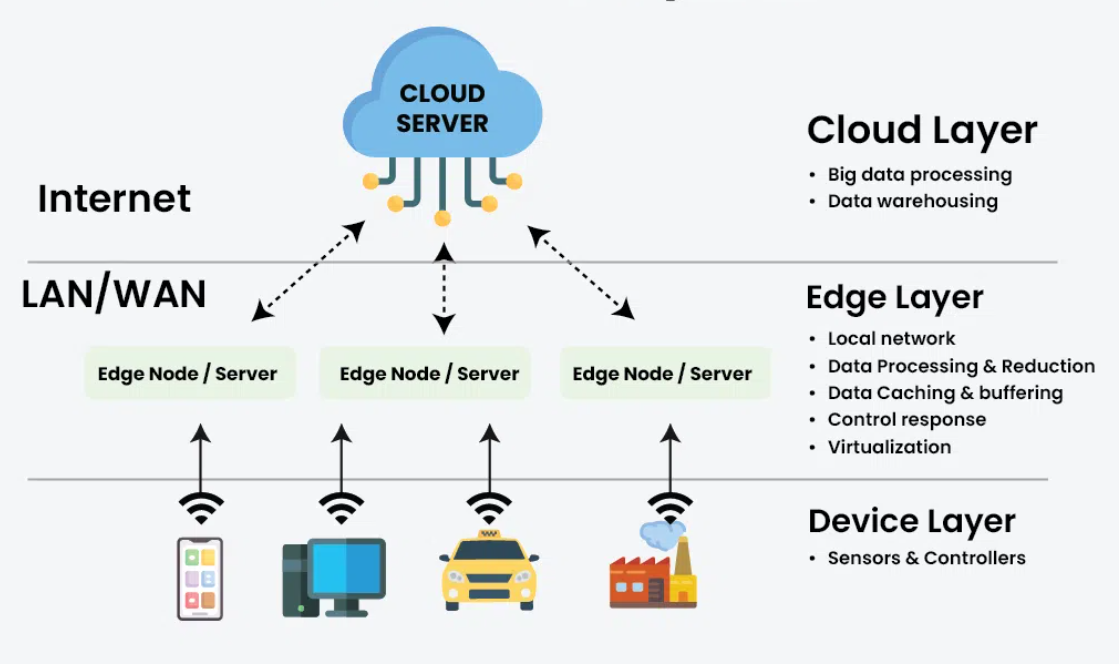
\includegraphics[width=0.9\textwidth]{graphics/Edge-Cloud-Architecture.png}
\caption{Sơ đồ kiến trúc Edge-Cloud Hybrid 3 tầng \cite{gfg_edge_cloud}}
\label{fig:edge-cloud-architecture}
\end{figure}

\paragraph*{Các thành phần cốt lõi}
\begin{enumerate}
    \item \textbf{Device Layer:}
    \begin{itemize}
        \item Các cảm biến, camera, PLC (Programmable Logic Controller) và cơ cấu chấp hành (actuators) ở điểm cực hạn. Chúng liên tục sinh ra lượng dữ liệu thô khổng lồ (Raw Data).
    \end{itemize}

    \item \textbf{Edge Layer:}
    \begin{itemize}
        \item Đóng vai trò là trung tâm thần kinh cục bộ. Phần cứng ở đây thường là các Industrial PC (IPC), Gateway, hoặc thiết bị nhúng mạnh mẽ (như NVIDIA Jetson).
        \item Chạy các phần mềm quản lý biên (như AWS IoT Greengrass, Azure IoT Edge).
        \item \textbf{Chức năng chính:} Tiền xử lý dữ liệu (lọc, nén, gộp), chạy quy tắc thời gian thực (Local Rules Engine), thực thi mô hình Machine Learning (AI Inference), và bảo mật cục bộ.
    \end{itemize}

    \item \textbf{Cloud Layer:}
    \begin{itemize}
        \item Đóng vai trò là trung tâm dữ liệu toàn cầu.
        \item \textbf{Chức năng chính:} Điều phối hàng triệu thiết bị, phân tích Big Data (Data Lake/Data Warehouse), huấn luyện mô hình ML (đưa các mô hình đã huấn luyện xuống Edge), và cung cấp Dashboard diện rộng.
    \end{itemize}
\end{enumerate}

\paragraph*{Cơ chế Đồng bộ hóa (Synchronization Patterns)}

\begin{table}[H]
\centering
\caption{Các cơ chế đồng bộ hóa trong kiến trúc Edge-Cloud Hybrid}
\begin{tabularx}{\textwidth}{c X X}
\toprule
\textbf{Cơ chế đồng bộ} & \textbf{Mô tả} & \textbf{Trường hợp sử dụng} \\
\hline
\textbf{Store-and-Forward}
  & Đệm dữ liệu cục bộ, gửi lên khi có kết nối.
  & Kết nối không ổn định (vệ tinh, 4G vùng sâu). \\
\hline
\textbf{Eventual Consistency}
  & Edge và Cloud hội tụ dần theo thời gian.
  & Telemetry không tới hạn (giám sát môi trường). \\
\hline
\textbf{Edge-First}
  & Edge tự ra quyết định, Cloud học từ kết quả.
  & Hệ thống an toàn thời gian thực (safety shutoff). \\
\hline
\textbf{Cloud-First}
  & Cloud ra quyết định, Edge thực thi lệnh.
  & Điều phối toàn bộ fleet (cập nhật firmware). \\
\hline
\textbf{Bi-directional Sync}
  & Cả Edge lẫn Cloud đều có thể thay đổi trạng thái.
  & Device Twin / Device Shadow (AWS/Azure). \\
\hline
\end{tabularx}
\end{table}

% --------------------------------------------------
\subsubsection{Phân tích sự đánh đổi}
\label{subsec:edge-cloud-tradeoff}

Triển khai Edge-Cloud là bài toán lớn về dòng tiền và năng lực kỹ thuật, đi kèm với những lợi thế và đánh đổi rõ rệt.

\begin{longtable}{c p{4cm} p{4cm} p{4cm}}

\caption{Phân tích đánh đổi kiến trúc Edge-Cloud Hybrid trong IoT} \\

\toprule
\textbf{Chiều Đánh Đổi} & \textbf{Ưu điểm} & \textbf{Hạn chế} & \textbf{Bối cảnh IoT cụ thể} \\
\midrule
\endfirsthead

\toprule
\textbf{Chiều Đánh Đổi} & \textbf{Ưu điểm} & \textbf{Hạn chế} & \textbf{Bối cảnh IoT cụ thể} \\
\midrule
\endhead

\bottomrule
\endlastfoot


\textbf{Latency}
  & Xử lý cục bộ: $<$~1ms on-device, $<$~10ms tại Edge Gateway.
  & Thêm một tầng kiến trúc cần quản lý và giám sát.
  & Ngắt khẩn cấp nhà máy không thể chờ round-trip Cloud (50--200ms); Edge phản ứng $<$~10ms. \\
\hline

\textbf{Reliability}
  & Tiếp tục vận hành khi Cloud không thể truy cập.
  & Đồng bộ sau khi kết nối lại rất phức tạp (conflict resolution, ordering, deduplication).
  & Nút lưới điện quản lý tải khi WAN bị ngắt. Dàn xếp 4 giờ sự kiện Edge với trạng thái Cloud cần thiết kế rất cẩn thận. \\
\hline

\textbf{Bandwidth}
  & Tổng hợp và lọc tại Edge --- chỉ gửi 1--5\% dữ liệu thô lên Cloud.
  & Phần cứng Edge (NVIDIA Jetson, IPC) tốn \$500--\$5,000+ mỗi site.
  & Nhà máy 500 camera: xử lý video tại Edge tiết kiệm 95\% băng thông Cloud. \\
\hline

\textbf{Data Sovereignty}
  & Dữ liệu nhạy cảm không bao giờ rời khỏi cơ sở.
  & Data residency đạt được bằng cấu hình, không phải kiến trúc --- cần kỷ luật vận hành.
  & Tuân thủ GDPR, HIPAA khi dữ liệu phải ở tại chỗ (on-premises / in-country). \\
\hline

\textbf{Security}
  & Phân đoạn mạng giới hạn bán kính tấn công khi bị xâm nhập.
  & Bảo mật vật lý Edge là trách nhiệm của nhà vận hành --- thiết bị có thể bị đánh cắp.
  & Kẻ tấn công có quyền truy cập vật lý vào Edge Gateway có thể trích xuất chứng chỉ Cloud backend. \\
\hline

\textbf{Complexity}
  & Công cụ phù hợp cho yêu cầu IoT doanh nghiệp phức tạp.
  & Mẫu phức tạp nhất --- cần chuyên môn về hệ thống phân tán, edge runtime (K3s, Greengrass), và giao thức đồng bộ.
  & Đội ngũ mới với IoT không nên bắt đầu từ đây --- đường cong học tập kéo chậm delivery hàng tháng. \\
\hline

\textbf{AI at the Edge}
  & ML inference trên thiết bị loại bỏ round-trip Cloud cho quyết định AI.
  & Cập nhật mô hình cần OTA delivery đến hàng nghìn node Edge.
  & YOLO object detection trên Jetson: 30fps cục bộ, không cần Cloud. Retrain và deploy mô hình mới đến 1,000 Edge node mất hàng giờ. \\

\end{longtable}

% --------------------------------------------------
\subsubsection{Ngữ cảnh áp dụng và Ngưỡng tới hạn}
\label{subsec:edge-cloud-thresholds}

Việc quyết định bao nhiêu phần trăm hệ thống đặt ở Edge và bao nhiêu phần đặt ở Cloud phụ thuộc vào các ngưỡng sau.

\paragraph*{Ngữ cảnh áp dụng lý tưởng}

\begin{enumerate}
    \item \textbf{Computer Vision \& Video Analytics:}
    Hàng trăm camera nhà máy đẩy video 4K sẽ đánh sập băng thông nội bộ. Edge Gateway chạy mô hình YOLO/SSD nhận diện lỗi ngay trên chuyền, chỉ gửi metadata (JSON): \texttt{\{"camera\_id": 04, "defect\_detected": "scratched\_surface", "timestamp": "..."\}}.

    \item \textbf{Cơ sở hạ tầng Thiết yếu \& Cận biên:}
    Gian khoan dầu ngoài khơi, tàu biển, mỏ khai thác sâu dưới lòng đất. Nơi kết nối vệ tinh đắt đỏ, chập chờn và dung lượng siêu thấp.

    \item \textbf{Tuân thủ Quyền riêng tư Y tế:}
    Hệ thống giám sát bệnh nhân trong phòng hồi sức. Dữ liệu nhịp tim phân tích tại giường bệnh, chỉ đẩy lên Cloud chỉ số sinh tồn đã ẩn danh hóa.
\end{enumerate}

\paragraph*{Ngưỡng tới hạn (Khi nào nên và không nên dùng Edge?)}

\begin{table}[H]
\centering
\caption{Ngưỡng tới hạn của kiến trúc Edge-Cloud Hybrid trong IoT}
\begin{tabularx}{\textwidth}{c X X X}
\toprule
\textbf{Ngưỡng} & \textbf{Giá trị tới hạn} & \textbf{Hậu quả khi vượt/không đạt ngưỡng} & \textbf{Giải pháp thay thế} \\
\hline
\textbf{Latency}
  & Ứng dụng yêu cầu $<$~50ms (closed-loop control).
  & Cloud-only bất khả thi --- round-trip Internet 50--200ms vi phạm chuẩn an toàn.
  & Edge \textbf{bắt buộc} cho vòng lặp kiểm soát. \\
\hline
\textbf{Bandwidth}
  & Ingestion rate $>$ năng lực uplink (VD: 10MB/s sinh ra vs 2MB/s uplink 4G).
  & Packet loss, queue overflow, hoặc hóa đơn Cloud bandwidth khổng lồ.
  & Triển khai Edge để nén, gộp (Batching) và chỉ gửi anomaly. \\
\hline
\textbf{Team Capability}
  & Đội ngũ chưa có kinh nghiệm hệ thống phân tán.
  & Lỗi đồng bộ (double-execution, lost updates) rất tinh vi và thảm khốc. Rollout OTA sai có thể brick hàng nghìn thiết bị.
  & Bắt đầu với Cloud-only + Rules Engine đơn giản. Thêm Edge khi đội ngũ trưởng thành. \\
\hline
\textbf{CapEx / ROI}
  & Dữ liệu giá trị thấp + Cloud bandwidth đủ rẻ.
  & Thêm Edge phức tạp hóa kiến trúc mà không mang lại lợi ích tương xứng (\$500--\$5,000+/site).
  & Giữ Cloud-only nếu dữ liệu không tới hạn và latency $>$~200ms được chấp nhận. \\
\hline
\end{tabularx}
\end{table}

% --------------------------------------------------
\subsubsection{Summary}
\label{subsec:edge-cloud-summary}

Kiến trúc lai Biên -- Đám mây (Edge-Cloud Hybrid) không phải là sự đánh đổi giữa hai mô hình, mà là \textbf{sự cộng sinh bắt buộc} để giải quyết các bài toán vật lý trong Công nghiệp 4.0. Đám mây mạnh về ``Trí tuệ tập thể toàn cầu'' (Global Intelligence) và ``Không gian vô hạn'', trong khi Biên chiến thắng tuyệt đối về ``Phản xạ thần kinh tức thì'' (Local Reflexes) và ``Sinh tồn độc lập'' (Survivability).

\noindent\textbf{Dùng Edge-Cloud Hybrid khi:}
\begin{itemize}
    \item Safety-critical IIoT cần phản hồi $<$~50ms
    \item Hoạt động offline là bắt buộc (remote sites, offshore, underground)
    \item Workload video/ảnh nặng --- băng thông uplink không đủ
    \item Tuân thủ data residency (GDPR, HIPAA) --- dữ liệu nhạy cảm không rời cơ sở
    \item Đội ngũ có kinh nghiệm hệ thống phân tán (5+ kỹ sư)
\end{itemize}

\noindent\textbf{Không dùng Edge-Cloud Hybrid khi:}
\begin{itemize}
    \item Đội ngũ chưa có kinh nghiệm distributed systems --- lỗi đồng bộ rất tinh vi
    \item CapEx hạn chế --- Edge hardware \$500--\$5,000+/site khó justify cho giám sát non-critical
    \item Dữ liệu giá trị thấp và Cloud bandwidth đủ rẻ --- thêm Edge là over-engineering
    \item Giai đoạn POC/MVP --- bắt đầu với Layered/Serverless rồi tiến hóa dần
\end{itemize}

Một hệ thống IoT trưởng thành hoạt động như một cơ thể người: Tầng Edge là tủy sống xử lý các phản xạ giật mình (shut-down máy móc tránh tai nạn trong 10ms) mà không cần chờ não bộ ra lệnh; còn Tầng Cloud là đại não, bình tĩnh tiếp nhận, tổng hợp dữ liệu toàn cầu để suy nghĩ chiến lược (phát hiện hao mòn máy móc để bảo trì dự đoán).
